% ============================================================
% Architecture diagram for the adaptive IoT defense framework
% Compile with:  pdflatex architecture_diagram.tex
% Output:        architecture_diagram.pdf
% ============================================================
\documentclass[border=4pt]{standalone}
\usepackage{amssymb}
\usepackage{tikz}
\usetikzlibrary{shapes.geometric, arrows.meta, positioning, fit, backgrounds, calc}

% ---- colour palette (greyscale-friendly) --------------------
\definecolor{colOffline}{RGB}{220,235,245}   % light blue  – offline stages
\definecolor{colOnline}{RGB}{220,245,220}    % light green – online RL loop
\definecolor{colBench}{RGB}{245,235,215}     % light amber – benchmark
\definecolor{colBorder}{RGB}{80,100,120}     % dark slate  – borders
\definecolor{colArrow}{RGB}{60,80,100}

% ---- common node styles -------------------------------------
\tikzset{
  box/.style={
    rectangle, rounded corners=3pt,
    draw=colBorder, line width=0.7pt,
    text centered, font=\small,
    inner sep=5pt, minimum height=1.8em
  },
  stageBox/.style={
    box,
    minimum width=3.6cm, minimum height=2.6cm,
    align=center
  },
  envBox/.style={
    box,
    minimum width=3.2cm, minimum height=2.0cm,
    align=center
  },
  groupLabel/.style={
    font=\small\bfseries, text=colBorder
  },
  arr/.style={
    -{Stealth[length=5pt]}, line width=0.8pt, color=colArrow
  },
  dasharr/.style={
    arr, dashed
  }
}

\begin{document}
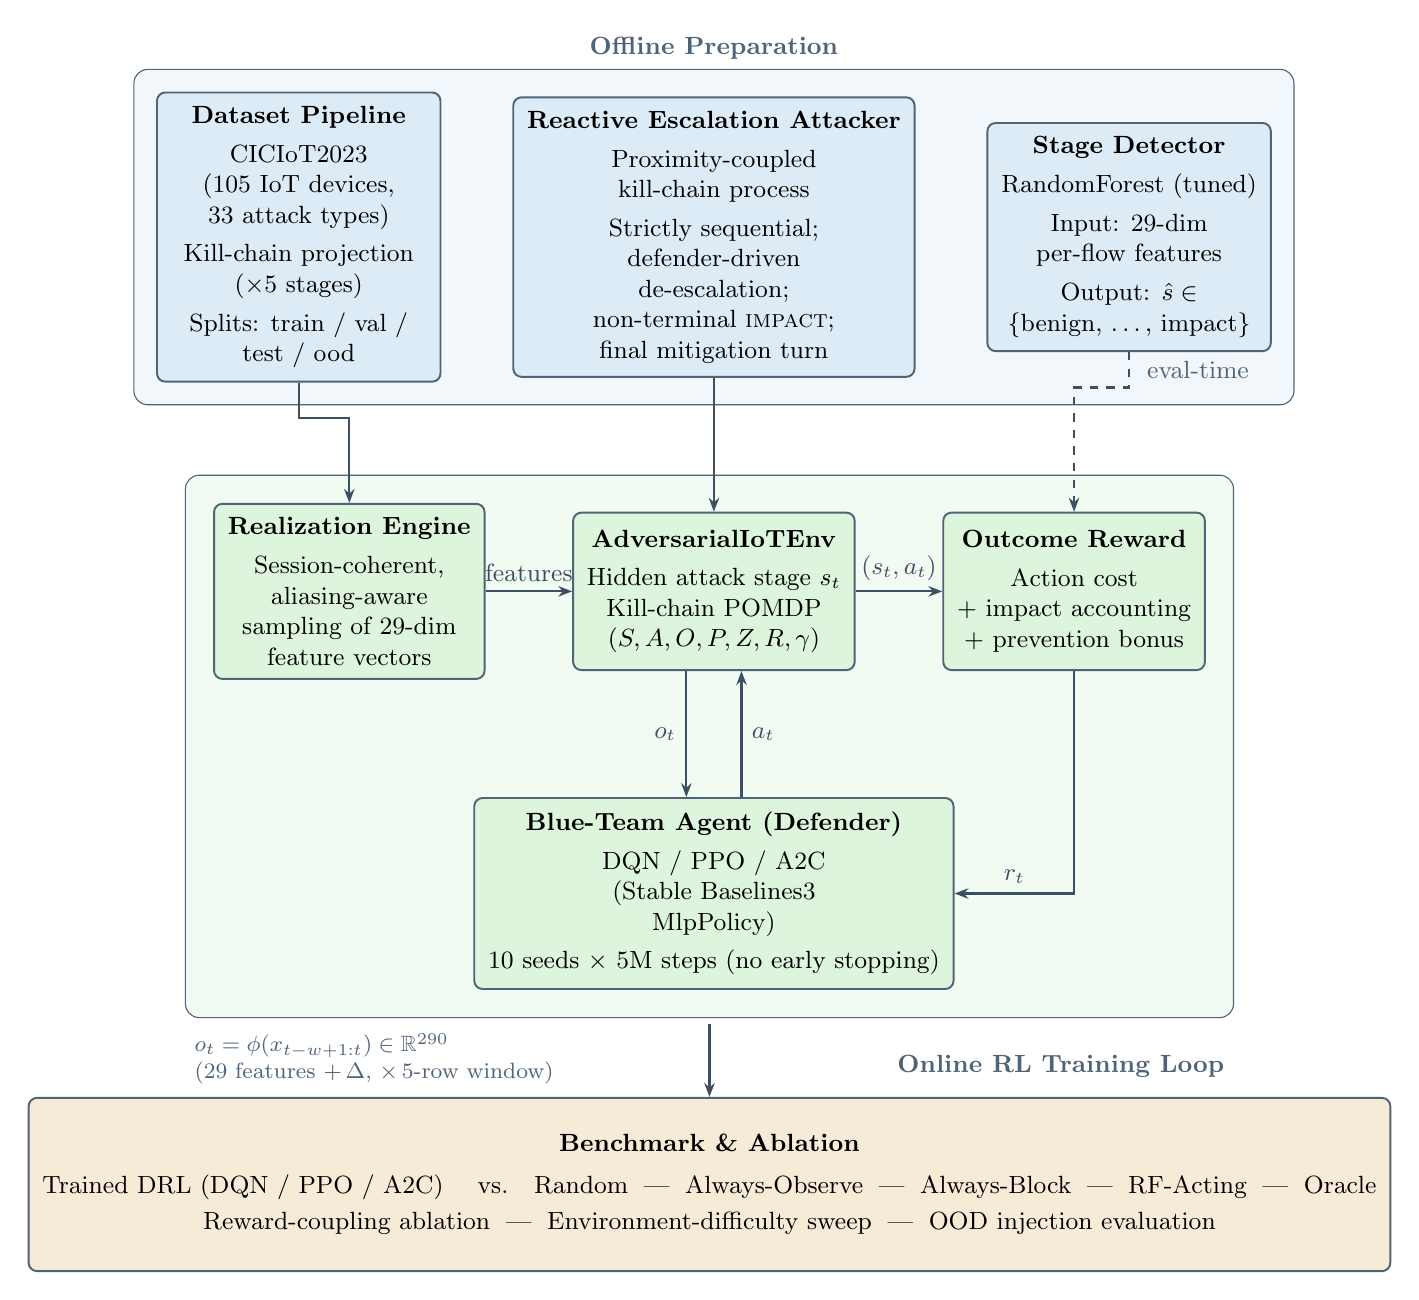
\begin{tikzpicture}[node distance=0.7cm and 0.9cm]

%% ==============================================================
%% Offline preparation lanes
%% ==============================================================

% --- Lane 1: Dataset pipeline ---
\node[stageBox, fill=colOffline] (dataset) {
  \textbf{Dataset Pipeline}\\[3pt]
  CICIoT2023\\
  (105 IoT devices,\\
   33 attack types)\\[3pt]
  Kill-chain projection\\
  ($\times$5 stages)\\[3pt]
  Splits: train / val /\\
  test / ood
};

% --- Lane 2: Reactive Escalation Attacker ---
\node[stageBox, fill=colOffline, right=of dataset] (redteam) {
  \textbf{Reactive Escalation Attacker}\\[3pt]
  Proximity-coupled\\
  kill-chain process\\[3pt]
  Strictly sequential;\\
  defender-driven\\
  de-escalation;\\
  non-terminal \textsc{impact};\\
  final mitigation turn
};

% --- Lane 3: Stage Detector ---
\node[stageBox, fill=colOffline, right=of redteam] (detector) {
  \textbf{Stage Detector}\\[3pt]
  RandomForest (tuned)\\[3pt]
  Input: 29-dim\\
  per-flow features\\[3pt]
  Output: $\hat{s} \in$\\
  \{benign, \ldots, impact\}
};

% --- Offline bounding box ---
\begin{scope}[on background layer]
  \node[draw=colBorder, fill=colOffline!40, rounded corners=5pt,
        inner sep=8pt,
        fit=(dataset)(detector),
        label={[groupLabel]above:Offline Preparation}] (stageI) {};
\end{scope}

%% ==============================================================
%% Online RL loop
%% ==============================================================

% --- Adversarial Environment ---
\node[envBox, fill=colOnline,
      below=1.7cm of redteam] (env) {
  \textbf{AdversarialIoTEnv}\\[3pt]
  Hidden attack stage $s_t$\\
  Kill-chain POMDP\\
  $(S,A,O,P,Z,R,\gamma)$
};

% --- Realization Engine ---
\node[envBox, fill=colOnline,
      left=1.1cm of env] (realizer) {
  \textbf{Realization Engine}\\[3pt]
  Session-coherent,\\
  aliasing-aware\\
  sampling of 29-dim\\
  feature vectors
};

% --- Reward function ---
\node[envBox, fill=colOnline,
      right=1.1cm of env] (reward) {
  \textbf{Outcome Reward}\\[3pt]
  Action cost\\
  + impact accounting\\
  + prevention bonus
};

% --- RL Agent ---
\node[envBox, fill=colOnline,
      below=1.6cm of env] (agent) {
  \textbf{Blue-Team Agent (Defender)}\\[3pt]
   DQN / PPO / A2C\\
   (Stable Baselines3\\
    MlpPolicy)\\[3pt]
  10 seeds $\times$ 5M steps (no early stopping)
};

% --- Online bounding box ---
\begin{scope}[on background layer]
  \node[draw=colBorder, fill=colOnline!40, rounded corners=5pt,
        inner sep=10pt,
        fit=(realizer)(reward)(agent)] (stageII) {};
\end{scope}
%% ==============================================================
%% Benchmark & Ablation
%% ==============================================================

\node[box, fill=colBench,
      minimum width=11.6cm, minimum height=2.2cm,
      align=center,
      below=1.0cm of stageII.south] (bench) {
  \textbf{Benchmark \& Ablation}\\[4pt]
  Trained DRL (DQN / PPO / A2C) \quad vs.\quad
  Random \;|\; Always-Observe \;|\; Always-Block \;|\; RF-Acting \;|\; Oracle\\[2pt]
  Reward-coupling ablation \;|\;
  Environment-difficulty sweep \;|\;
  OOD injection evaluation
};

%% ==============================================================
%%  ARROWS
%% ==============================================================

% Dataset to realizer
\draw[arr] (dataset.south) -- ++(0,-0.45) -| (realizer.north);

% Markov attacker to env
\draw[arr] (redteam.south) -- (env.north);

% Detector to reward, dashed = eval-time only
\draw[dasharr] (detector.south) -- ++(0,-0.45) -| (reward.north);
\node[font=\small, text=colBorder, anchor=west]
    at ([xshift=3pt,yshift=-0.22cm]detector.south) {eval-time};

% Realizer → Env (sampled feature rows feed the environment)
\draw[arr] (realizer.east) -- node[above, font=\small]{features} (env.west);

% Env → Reward (transition consequence)
\draw[arr] (env.east) -- node[above, font=\small]{$(s_t,a_t)$} (reward.west);

% Reward → Agent (scalar reward)
\draw[arr] (reward.south) |- (agent.east)
    node[near end, above, font=\small]{$r_t$};

% Env → Agent (observation, left half of the vertical channel)
\draw[arr] ([xshift=-0.35cm]env.south) -- node[left, font=\small]{$o_t$}
    ([xshift=-0.35cm]agent.north);

% Agent → Env (action, right half of the vertical channel)
\draw[arr] ([xshift=0.35cm]agent.north) -- node[right, font=\small]{$a_t$}
    ([xshift=0.35cm]env.south);

% Online loop to benchmark
\draw[arr] ([yshift=-2pt]stageII.south) -- (bench.north);

%% ==============================================================
%%  OBSERVATION label
%% ==============================================================
\node[font=\footnotesize, align=left, text=colBorder,
      below right=2pt and 0pt of stageII.south west, anchor=north west] {
  $o_t = \phi(x_{t-w+1:t}) \in \mathbb{R}^{290}$\\
  (29 features $+\,\Delta$, $\times\,5$-row window)
};
\node[groupLabel, below left=10pt and 0pt of stageII.south east,
      anchor=north east] {Online RL Training Loop};

\end{tikzpicture}
\end{document}
